\section{Introduction}
\begin{frame}[allowframebreaks]
	\frametitle{Introduction}
	
	\par The databse and sources used in this work are available in \url{https://github.com/ensismoebius/deepLearnning}):\newline
	
	\par Spiking Neural Networks (SNNs) mimic in some degree the workings of the brain by utilizing action potentials, in contrast to continuous values transmitted between neurons in more traditional neural networks.\newline
	
	\par The term "Spiking" originates from the behavior of biological neurons, which sporadically emit action potentials, creating voltage spikes that convey information \cite{kasabov2019time}. Figure \ref{fig:neuronspikes} illustrates these spikes.\newline
	
	\par An SNN \textbf{is not} a one-to-one simulation of neurons. Instead, it approximates certain computational capabilities of specific biological properties. Some studies like \cite{jones2020single} created models closer to natural neurons exploring the nonlinearity of dendrites and other neuron features yielding remarkable results in the classification.
	
	\begin{figure}[H]
		\centering
		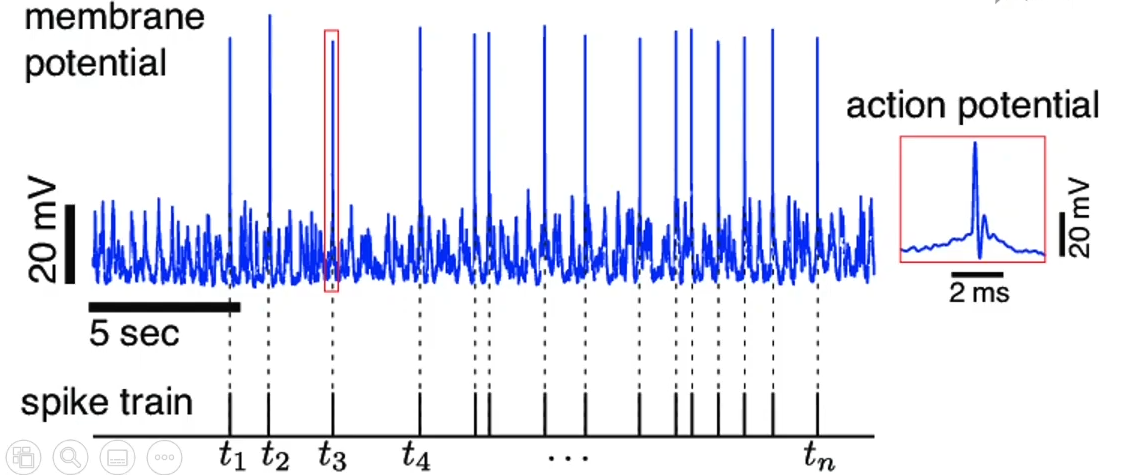
\includegraphics[width=.8\linewidth]{images/neuronSpikes}
		\caption{Spikes from a noisy signal. Source \cite{dan_goodman_2022_7044500}}
		\label{fig:neuronspikes}
	\end{figure}
\end{frame}

\section{Characteristics}
\begin{frame}[allowframebreaks]
	\frametitle{General characteristics}
	
	\par SNNs possess several noteworthy characteristics that distinguish them from traditional machine learning techniques, including classical neural networks. These distinctions encompass \cite{kasabov2019time}:
	
	\begin{itemize}
		\item Proficiency in modeling temporal, spatial-temporal, or spectro-temporal data.
		\item Effectiveness in capturing processes involving various time scales.
		\item Seamless integration of multiple modalities, such as sound and vision, into a unified system.
		\item Aptitude for predictive modeling and event prediction.
		\item Swift and highly parallel information processing capabilities.
		\item Streamlined information processing.
		\item Scalability, accommodating structures ranging from a few tens to billions of spiking neurons.
		\item Minimal energy consumption when implemented on neuromorphic platforms.
	\end{itemize}

	\begin{figure}
		\centering
		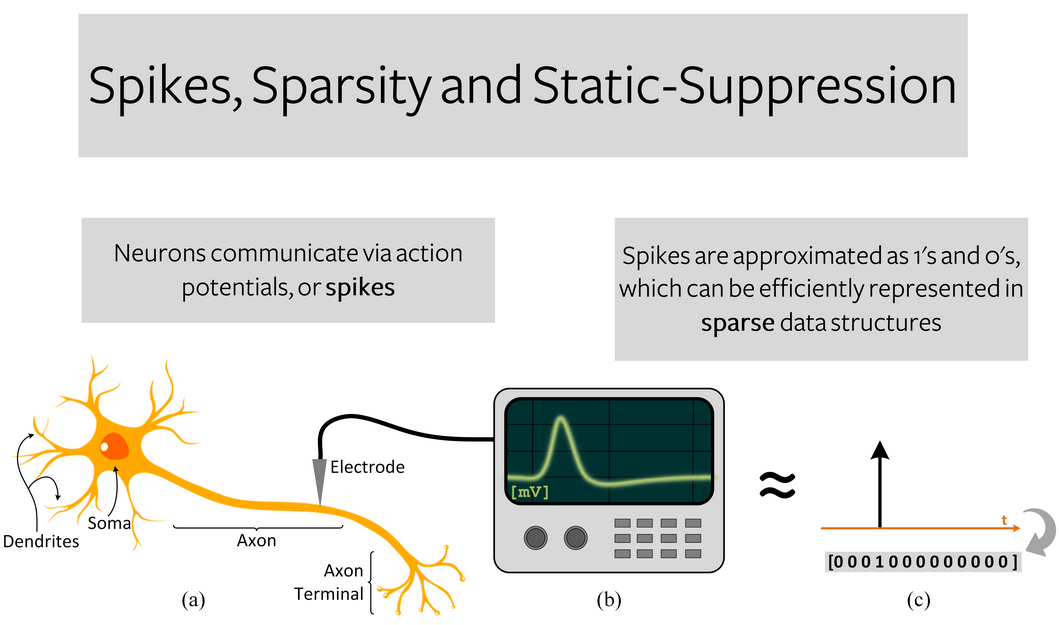
\includegraphics[width=0.7\linewidth]{images/spikesSparsityStaticSupress}
		\caption{Sparsity on Spike Neuron Networks. Source: \cite{10242251}}
		\label{fig:spikessparsitystaticsupress}
	\end{figure}
	

\end{frame}

\begin{frame}[allowframebreaks]
	\frametitle{Energy characteristics}
	
		\par Spiking Neural Networks (SNNs) are often considered power-efficient for several reasons:
		
		\par \textbf{Event-Driven Processing}: SNNs are inherently event-driven. Instead of constantly updating neuron activations and synapse weights as in traditional artificial neural networks (ANNs), SNNs only transmit spikes (action potentials) when a neuron's membrane potential reaches a certain threshold. This event-driven approach reduces the amount of computation required and can lead to significant energy savings.
		
		\par \textbf{Sparse Activity}: SNNs tend to exhibit sparse activity, meaning that only a small percentage of neurons are active at any given time. This sparsity reduces the number of computations that need to be performed, which is especially beneficial for hardware implementations where most of the energy consumption comes from active components. See Figure \ref{fig:sparsity}.
		
		\par \textbf{Low Precision}: SNNs can often work with lower precision than ANNs. While ANNs typically use high-precision floating-point numbers for neuron activations and synaptic weights, SNNs can use lower precision fixed-point or binary representations. Lower precision computations require less energy to perform.
		
		\par \textbf{Neuromorphic Hardware}: SNNs can be efficiently implemented on specialized neuromorphic hardware, which is designed to mimic the energy-efficient behavior of biological neural systems. These hardware platforms are optimized for the event-driven nature of SNNs, further reducing power consumption.
		
		\par \textbf{Energy-Aware Learning Rules}: SNNs can employ learning rules that take into account energy efficiency. For example, some learning rules prioritize strengthening or weakening synapses based on their contribution to network activity, which can lead to more energy-efficient learning.
		
		\par \textbf{Spike Encoding}: SNNs can encode information in the timing and frequency of spikes, which can be a highly efficient way to represent and process data, particularly for event-based sensors like vision sensors or auditory sensors.
		
		\begin{figure}
			\centering
			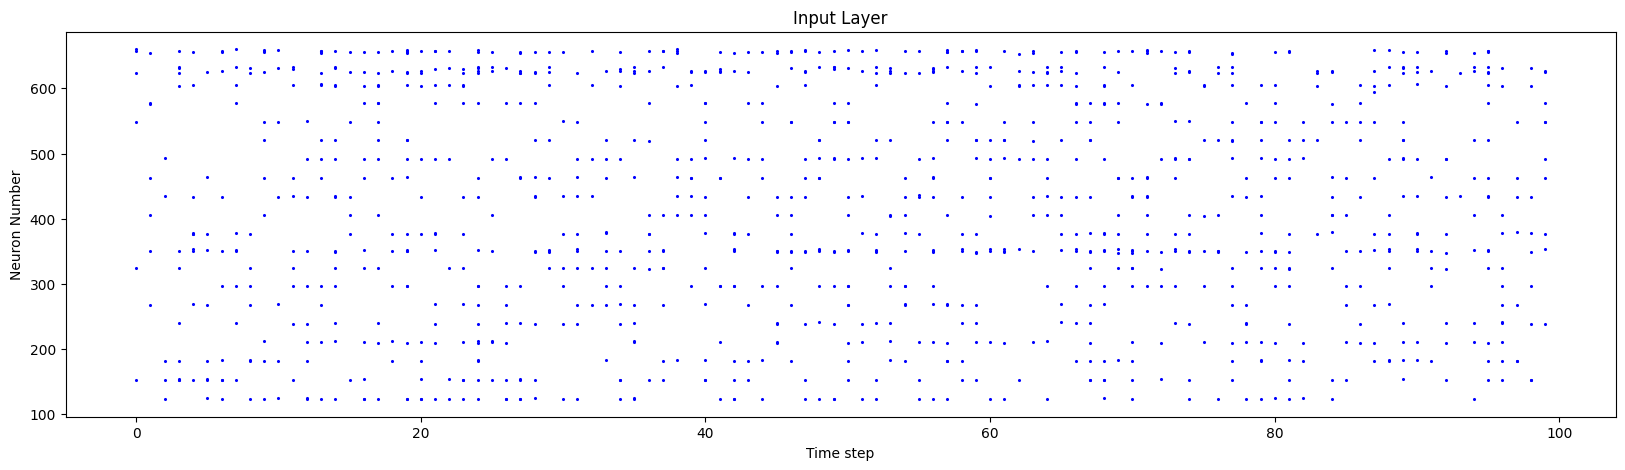
\includegraphics[width=\linewidth]{images/sparsity}
			\caption{Sparse activity of a SNN}
			\label{fig:sparsity}
		\end{figure}
		
\end{frame}

\section{Theory}
\begin{frame}[allowframebreaks]
	\frametitle{Theory: Spikes and potentials}
	
	\begin{columns}
		\column{0.5\textwidth}
			\par In order to emulate such behavior, let's begin with a simple model: The "Leaky Integrate and Fire neuron" (LIF). The LIF model describes the evolution of membrane potential which the potential decay over time.
			\begin{equation}
				\tau \cdot \frac{dV}{dt} = -V
				\label{eq:leak}
			\end{equation}
			
			\par When a neuron receives a spike, the membrane potential $V$ increases according to a synaptic weight $w$.
			\begin{equation}
				V = V + w
			\end{equation}
			
			\par Such behaviors are depicted in Figure \ref{fig:neuronspikes2}.
		\column{0.5\textwidth}
			\begin{figure}
				\centering
				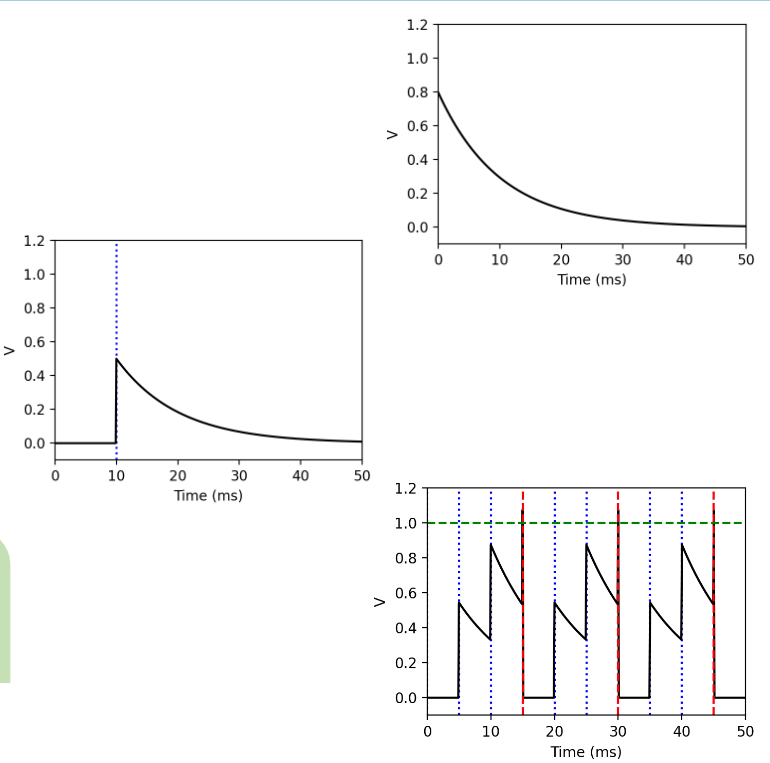
\includegraphics[width=.87\linewidth]{images/neuronSpikes2}
				\caption{Evolution of a Spike. Source \cite{dan_goodman_2022_7044500}}
				\label{fig:neuronspikes2}
			\end{figure}
	\end{columns}

	\begin{columns}
	\column{0.5\textwidth}
		\par A spike neuron acts like an \textbf{resistor-capacitor} circuit (RC).
		\begin{figure}
			\centering
			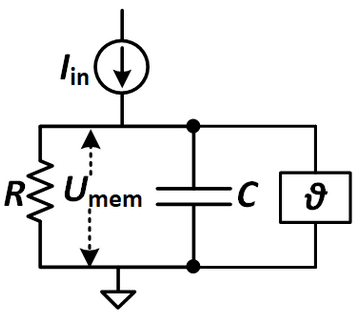
\includegraphics[width=0.6\linewidth]{images/rcmodel}
			\caption[RC model]{Resistor-capacitor circuit model. Source: \cite{10242251}}
			\label{fig:rcmodel}
		\end{figure}
	\column{0.5\textwidth}
		\begin{lstlisting}[language=Python, caption="Code for RC model"]
def convert_to_time(data, tau=5, threshold=0.01):
	spike_time = tau * torch.log(data / (data - threshold))
	return spike_time
\end{lstlisting}

		\begin{figure}
			\centering
			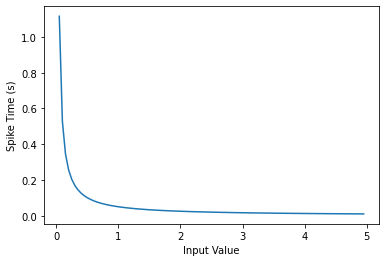
\includegraphics[width=0.7\linewidth]{images/rcmodelplot}
			\caption{The smaller the value, the later the spike occurs with exponential dependence}
			\label{fig:rcmodelplot}
		\end{figure}
		
	\end{columns}

	\begin{lstlisting}[language=Python]

class Neuron:
    """
    Leak integrate and fire neuron - LIF

    """
    def __init__(self, tau=10, threshold=1):

        # Initial membrane voltage
        self.voltage = 0

        # The smaller tau is the faster the voltage decays
        # When tau is large the neuron acts as an intergrator summing its inputs
        # and firing when a certain threshold is reached.
        # When tau is small the neuron acts as a coincidence detector, firing a
        # spike only when two or more input arrive simultaneosly.
        self.tau = tau

        # The threshold above which the neuron fires
        self.threshold = threshold

        # Time step for decaying (i still don't known what this really is)
        # Bigger the number faster the decay
        self.timeStep = 0.5

        # The rate by which the membrane voltage decays each time step
        self.alpha = np.exp(-self.timeStep/self.tau)

    def set_tau(self, tau):
        self.tau = tau
        self.alpha = np.exp(-self.timeStep/self.tau)

    def fire_spike(self):
        if self.voltage > self.threshold:
            self.voltage = 0
            return 1
        return 0

    def add_synaptic_weight(self, weigth):
        # Membrane voltage integration
        self.voltage += weigth

    def iterate(self):
        # Membrane voltage leak
        self.voltage = max(self.voltage * self.alpha, 0)
        return self.fire_spike()
\end{lstlisting}
\end{frame}

\begin{frame}[allowframebreaks]
	\frametitle{Demonstration: Simulating a spike neuron}
	\begin{figure}
		\centering
		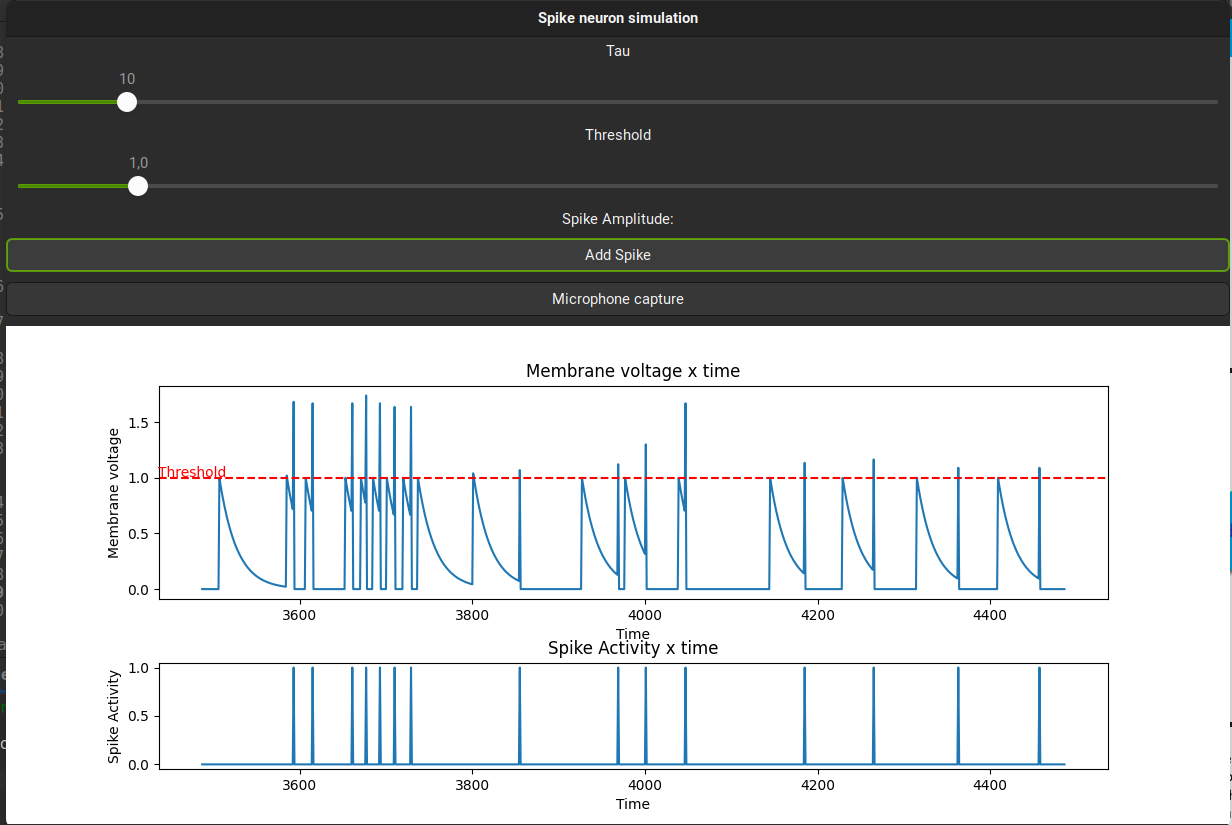
\includegraphics[width=0.6\linewidth]{images/spikeNeuronSimulation}
		\caption[Spiking Neuron Simulator]{A simulation a of spiking neuron}
		\label{fig:spikeneuronsimulation}
	\end{figure}
\end{frame}

\begin{frame}
	\frametitle{Theory: Training overview}
	\par As shown in Figure \ref{fig:neuronspikes2}, when a neuron reaches a certain threshold, it resets ($V = 0$). Note that $V=0$ is just one of the possible values of reset, after this the neuron may or may not enter in a refractory period. \textbf{These, an another values cited ahead, can be parameterized or learned}.\newline
	
	\par \textbf{How do SNNs get trained?} Well, this is still an open question. An SNN neuron has an activation-function behavior that is more relatable to a \textbf{step function}. Therefore, in principle, we can't use gradient descent-based solutions because this kind of function \textbf{is not} differentiable \cite{kasabov2019time}.\newline
	
	\par But there are some insights out there that may shed some light on this subject: While some \textit{in vivo/in vitro} observations show that brains, in general, learn by strengthening/weakening and adding/removing synapses or even by creating new neurons or other cumbersome methods like RNA packets, there are some more acceptable ones like the ones in the slide \cite{kasabov2019time}:

\end{frame}

\begin{frame}
	\frametitle{Theory: Training overview}
	\begin{itemize}
		\item Spike Timing-Dependent Plasticity (STDP): The idea is that if a pre-synaptic neuron fires \textbf{before} the post-synaptic one, there is a strengthening in connection, but if the post-synaptic neuron fires before, then there is a weakening.
		\item Surrogate Gradient Descent: The technique \textbf{approximates} the step function by using another mathematical function, which is differentiable (like a sigmoid), in order to train the network. These approximations are used only \textbf{in the backward pass}, while keeping the step function in the forward pass \cite{kasabov2019time}.
		\item Evolving Algorithms: Use the selection of the fittest throughout many generations of networks.
		\item Reservoir/Dynamic Computing: \textbf{Echo state networks} or \textbf{Liquid state machines} respectively. These will be discussed further in this presentation.
	\end{itemize}
\end{frame}

\begin{frame}
	\frametitle{Theory: Surrogate gradient descent}
		\begin{columns}
		\column{0.5\textwidth}
			\par Gradient descent is a well known method to adjust the weights of a network, however it can't be used \textbf{directly} in SNNs because its behavior on activation obeys a \textbf{Heaviside function} which is not differentiable and its gradients are all zero.\newline
			
			\par \textbf{Surrogate gradient descent} is a method in which the derivative of the \textit{sigmoid} or another similar function is used just in the \textbf{backward pass}.
			
			\begin{lstlisting}[language=Python, caption={Surrogate in snnTorch}]
from snntorch import surrogate
spike_grad = surrogate.fast_sigmoid() 
\end{lstlisting}
		\column{0.5\textwidth}
			\begin{figure}
				\centering
				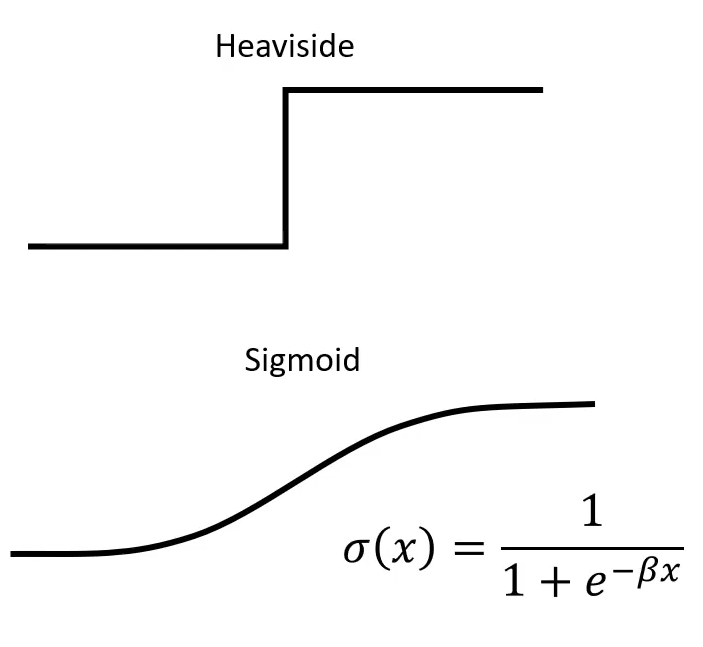
\includegraphics[width=0.9\linewidth]{images/heavisideSigmoid}
				\caption{Heaviside sigmoid functions plots}
				\label{fig:heavisidesigmoid}
			\end{figure}
	\end{columns}
\end{frame}

\begin{frame}[allowframebreaks]
	\frametitle{Theory: Coding}
	\begin{columns}
		\column{0.3\textwidth}
			\par Despite SNNs can work in conjunction with another types of layers in deep networks they are made to exploit data that varies in time (audio, videos etc.) then, sometimes we need to make some static data be presented in time-varying fashion.\newline
			
			\par For now and according to \cite{10242251} there is three ways to do this:
		\column{0.4\textwidth}
			\begin{itemize}
				\item \textbf{rate coding}: Data with higher values spikes more than data with lesser values. Not so power efficient but very robust to noise.
				\item \textbf{latency coding}: Data with higher values spikes first, data with lesser values spikes last. Very power efficient but not so good against noise.
				\item \textbf{delta modulation}: Changes in data creates spikes. Good to detect movement but very prone to noises.
			\end{itemize}
		\column{0.2\textwidth}
			\begin{figure}
				\centering
				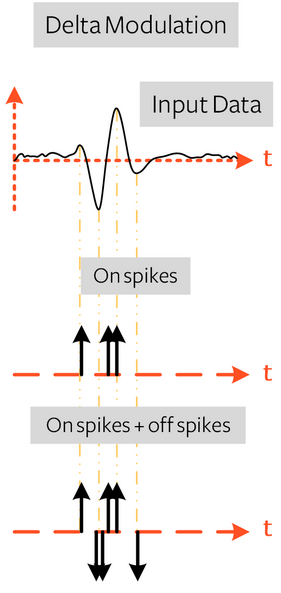
\includegraphics[width=\linewidth]{images/deltaModulation}
				\caption{Delta modulation}
				\label{fig:deltamodulation}
			\end{figure}
	\end{columns}

	\begin{itemize}
		\item \textbf{Rate coding}: \href{./videos/mnist_rate.mp4}{mnist\_rate.mp4}
		\item \textbf{Latency coding} \href{./videos/mnist_latency.mp4}{mnist\_latency.mp4}
	\end{itemize}
\end{frame}


\section{Experiments}
\begin{frame}
	\frametitle{Experiment: Architecture}
	\begin{columns}
		\column{.2\textwidth}
			\par The experiments objective is to compare a convolutional neural network (CNN) with an SNN.
			\par The chosen architecture was the following:
		\column{.8\textwidth}
		
		\only<1>{
			\framesubtitle{CNN architecture}
			\begin{figure}
				\centering
				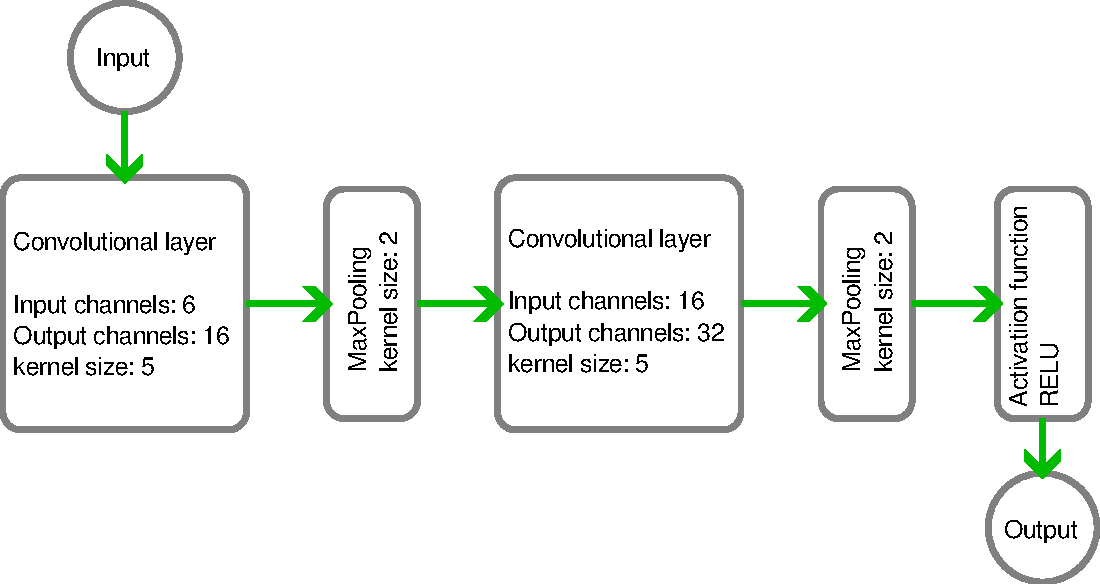
\includegraphics[width=\linewidth]{images/architectureCNN}
				\caption{Convolutional neural network architecture}
				\label{fig:architecturecnn}
			\end{figure}
		}
		\only<2>{
			\framesubtitle{SNN architecture}
			\begin{figure}
				\centering
				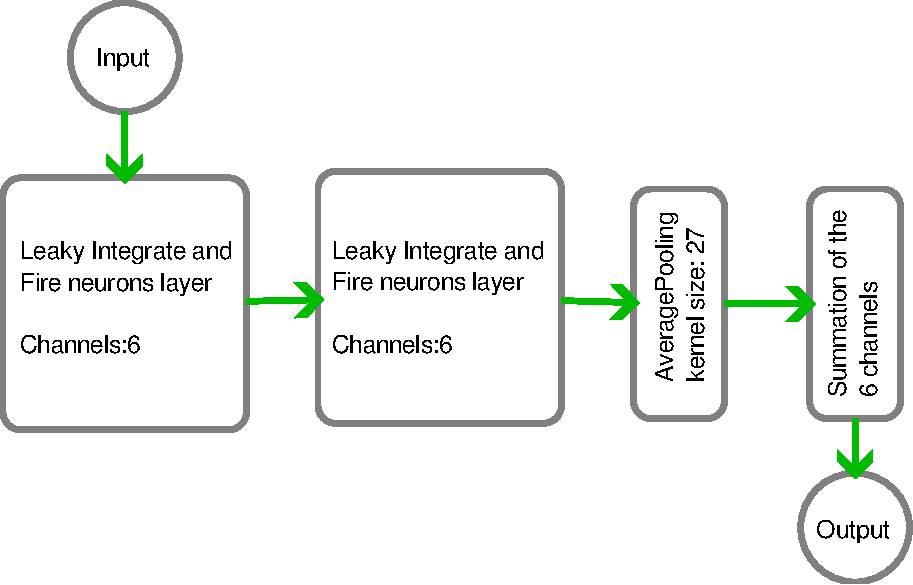
\includegraphics[width=.85\linewidth]{images/architectureSNN}
				\caption{Spiking neural network architecture}
				\label{fig:architecturesnn}
			\end{figure}
		}
	\end{columns}
\end{frame}

\begin{frame}
	\frametitle{Experiment: Architecture}
	\framesubtitle{Code architecture}
	\par The code can be found at \href{https://github.com/ensismoebius/deepLearnning/tree/main/simulations/article}{simulations/article} folder in Google collab notebook format or in pure Python.
	\begin{columns}
		\begin{column}{0.5\textwidth}
			\par The SNN and CNN was trained according to the following parameters:
			\begin{itemize}
				\item \textbf{batch size}: 10
				\item \textbf{number of epochs}: 100
			\end{itemize}
			
			\par Some parameters are exclusive to SNNs like:
			
			\begin{itemize}
				\item \textbf{insist}: 4 (amount of times the same data is presented to the network)
				\item \textbf{neuron decay rate}: 0.9 (the rate LIF neuron loses its voltage)
			\end{itemize}	
		\end{column}
		\begin{column}{0.5\textwidth}
			\only<1>{
				\begin{lstlisting}[language=Python, caption={CNN architecture}]

self.model = nn.Sequential(
	nn.Conv1d(in_channels=6, 
		out_channels=16, kernel_size=5
	),
	nn.MaxPool1d(kernel_size=2),
	
	nn.Conv1d(in_channels=16,
		out_channels=32, kernel_size=5
	),
	nn.MaxPool1d(kernel_size=2),
	
	nn.Flatten(),
	nn.Linear(feature_size, 128),
	nn.ReLU(),
	nn.Linear(128, 27)
)
\end{lstlisting}
			}
			\only<2>{
				\begin{lstlisting}[language=Python, caption={SNN architecture}]
self.model = nn.Sequential(
	nn.Linear(inputLength, 4096),
	snn.Leaky(
		beta=neuronDecayRate, 
		spike_grad=spike_grad
	),
	nn.Linear(4096, 27),
	snn.Leaky(
		beta=neuronDecayRate, 
		spike_grad=spike_grad
	),
	nn.AvgPool1d(27, stride=1)
)
\end{lstlisting}
			}
		\end{column}
	\end{columns}
\end{frame}

\begin{frame}[allowframebreaks]
	\frametitle{Experiment: Database}
   	\begin{columns}
    	\begin{column}{0.5\textwidth}
			\par The used  database \cite{PRG16} can be found at \href{https://sinc.unl.edu.ar/grants/brain-computer-interfaces/}{https://sinc.unl.edu.ar/grants/brain-computer-interfaces} and consists in a set of EEG data recorded with 6 electrodes during a imagined speech of the words in spanish: 
		    "A", "E", "I", "O", "U", "Arriba", "Abajo", "Adelante", "Atrás", "Derecha", "Izquierda".\newline
		    
		    \par Each channel captured 4096 samples and has the following ids: 'F3','F4', 'C3', 'C4', 'P3', 'P4' according to 10-20 system \cite{ScienceOpenVid:5960cfa8-7fde-441c-8592-35fdb9841499}.
    	\end{column}
    	\begin{column}{0.5\textwidth}
    		\begin{figure}
    			\centering
    			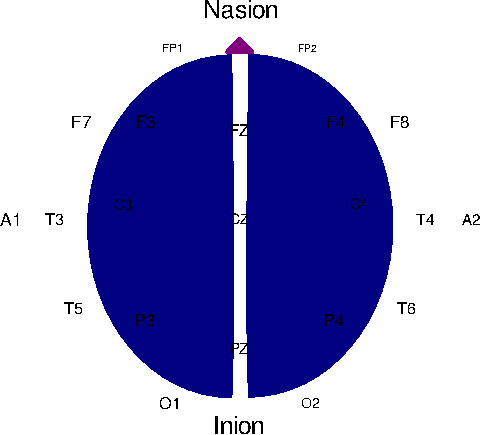
\includegraphics[width=\linewidth]{images/sistema10-20}
    			\caption{10-20 system. Source: \cite{sistema10-20}}
    			\label{fig:sistema10-20}
    		\end{figure}
    	\end{column}
    \end{columns}

	\begin{figure}
		\centering
		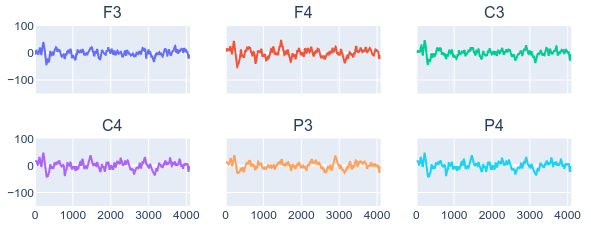
\includegraphics[width=\linewidth]{images/dataBaseSample}
		\caption{Sample of data from database}
		\label{fig:databasesample}
	\end{figure}
\end{frame}

\begin{frame}
	\frametitle{Experiment: Results}
	\begin{columns}
		\begin{column}{0.5\textwidth}
			\begin{figure}
				\centering
				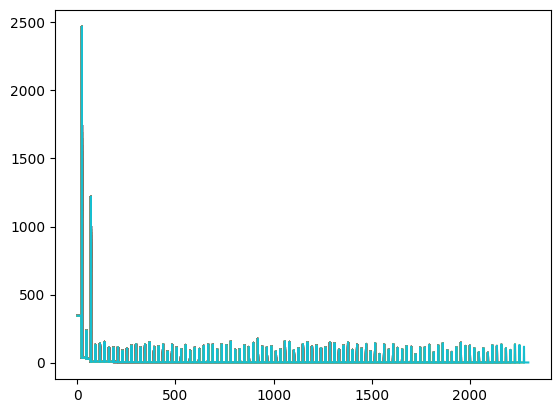
\includegraphics[width=\linewidth]{images/cnnResults}
				\caption[CNN Results]{CNN Results. The horizontal axis represents iterations, vertical the loss }
				\label{fig:cnnresults}
			\end{figure}
			
		\end{column}
		\begin{column}{0.5\textwidth}
			\begin{figure}
				\centering
				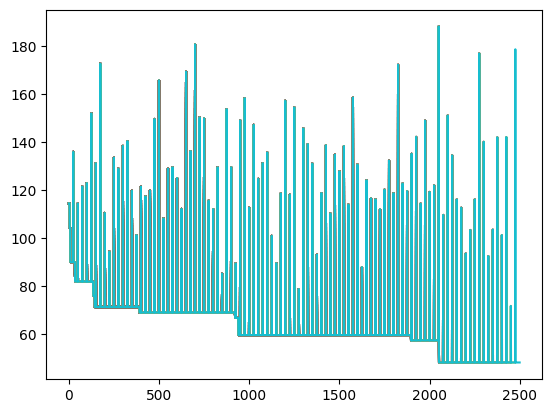
\includegraphics[width=\linewidth]{images/snnResults}
				\caption[SNN Results]{SNN Results. The horizontal axis represents iterations, vertical the loss }
				\label{fig:snnresults}
			\end{figure}
		\end{column}
	\end{columns}
\end{frame}
